% ============================================================================
%  fig_cronograma.tex - Cronograma de la propuesta (S1–S4) frente al avance real
%  Pong en FPGA - Electrónica Digital 1 - UNAL
%  Juan David Ortiz Muñoz, David Eduardo Chivata Arias, Daniel Felipe Castro González
%  Compilar con: pdflatex fig_cronograma.tex
% ============================================================================
\documentclass[border=6pt]{standalone}
\usepackage[utf8]{inputenc}
\usepackage[T1]{fontenc}
\usepackage{lmodern}
\usepackage{tikz}
\begin{document}
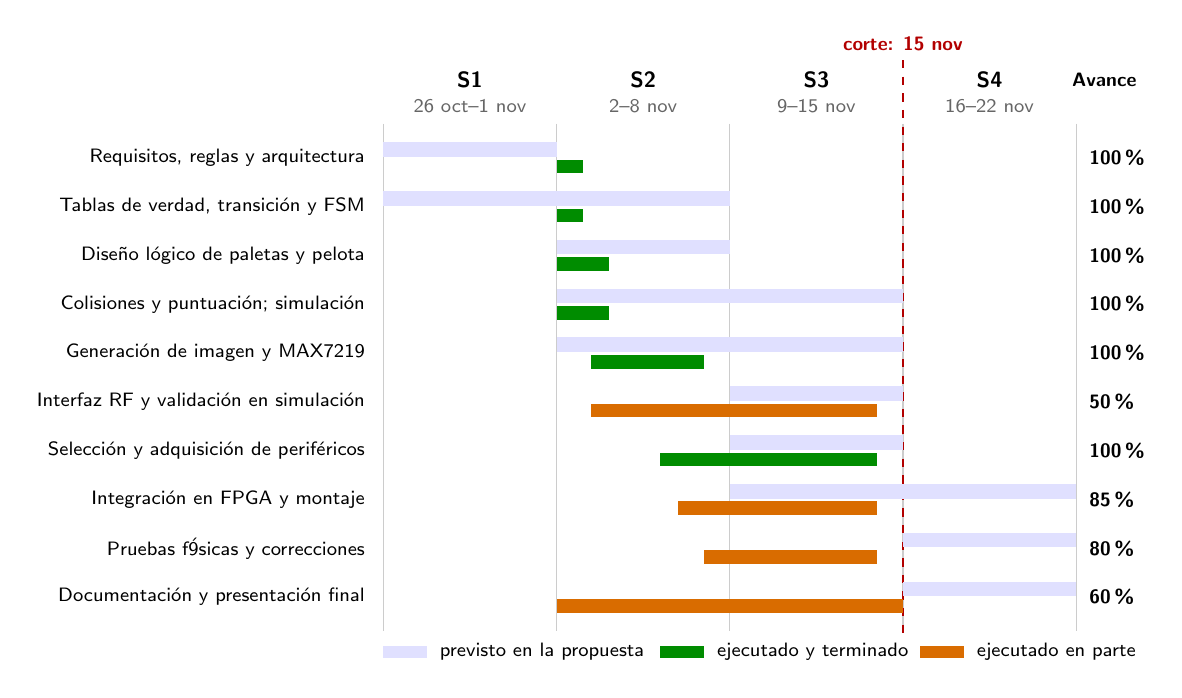
\begin{tikzpicture}[font=\sffamily\scriptsize, x=2.2cm, y=0.62cm]
  % Encabezado de semanas
  \foreach \s/\f [count=\i from 0] in {S1/26 oct–1 nov, S2/2–8 nov, S3/9–15 nov, S4/16–22 nov}{
    \node[font=\sffamily\footnotesize\bfseries] at (\i+0.5, 1.1) {\s};
    \node[text=black!60] at (\i+0.5, 0.55) {\f};
    \draw[black!20] (\i, 0.2) -- (\i, -10.2);
  }
  \draw[black!20] (4, 0.2) -- (4, -10.2);
  % Fecha de corte del informe de avance: 15 de noviembre (fin de S3)
  \draw[red!70!black, dashed, line width=0.8pt] (3, 1.5) -- (3, -10.3);
  \node[red!70!black, anchor=south, font=\sffamily\scriptsize\bfseries] at (3, 1.5) {corte: 15 nov};

  % actividad / inicio previsto / fin previsto / inicio real / fin real / avance / color
  \foreach \t/\pa/\pb/\ra/\rb/\av [count=\i from 1] in {
      Requisitos{,} reglas y arquitectura/0/1/1/1.15/100,
      Tablas de verdad{,} transición y FSM/0/2/1/1.15/100,
      Diseño lógico de paletas y pelota/1/2/1/1.3/100,
      Colisiones y puntuación; simulación/1/3/1/1.3/100,
      Generación de imagen y MAX7219/1/3/1.2/1.85/100,
      Interfaz RF y validación en simulación/2/3/1.2/2.85/50,
      Selección y adquisición de periféricos/2/3/1.6/2.85/100,
      Integración en FPGA y montaje/2/4/1.7/2.85/85,
      Pruebas físicas y correcciones/3/4/1.85/2.85/80,
      Documentación y presentación final/3/4/1/3/60}{
    \pgfmathsetmacro{\y}{-\i+0.5}
    \node[anchor=east, align=right] at (-0.05, \y) {\t};
    \fill[blue!12] (\pa, \y+0.02) rectangle (\pb, \y+0.32);
    \ifnum\av=100
      \fill[green!55!black] (\ra, \y-0.32) rectangle (\rb, \y-0.04);
    \else
      \fill[orange!85!black] (\ra, \y-0.32) rectangle (\rb, \y-0.04);
    \fi
    \node[anchor=west, font=\sffamily\scriptsize\bfseries] at (4.02, \y) {\av\,\%};
  }
  \node[anchor=west, font=\sffamily\scriptsize\bfseries] at (3.92, 1.1) {Avance};

  % Leyenda
  \fill[blue!12] (0, -10.75) rectangle (0.25, -10.5); \node[anchor=west] at (0.27, -10.62) {previsto en la propuesta};
  \fill[green!55!black] (1.6, -10.75) rectangle (1.85, -10.5); \node[anchor=west] at (1.87, -10.62) {ejecutado y terminado};
  \fill[orange!85!black] (3.1, -10.75) rectangle (3.35, -10.5); \node[anchor=west] at (3.37, -10.62) {ejecutado en parte};
\end{tikzpicture}
\end{document}
